\chapter{Modélisation}

\section{Introduction}

Dans ce chapitre, on va étudier les approches faites dans la conception et implémentation des réseaux de neurones binaires,  dériver les formules nécessaires dans les cas des couches dense et convolutionnelles, et dans le cas générique.

\subsection{Importance de ce chapitre}
Dans les articles de BNNs considérés, les formules données ne sont généralement applicable qu'aux couches convolutionnelles à $2$ dimensions.
\newline Nous chercherons ici à trouver une approche générique avec laquelle on peut dériver pour chaque modèle considéré les équations des couches dense, convolutionnelles, récurrentes, etc...
\newline Notre approche admet principalement $2$ caractéristiques:
\subsubsection{Rigueur}
Pour établir les équations nécessaires, nous avons suivi les étapes suivantes:
\begin{enumerate}
	\item Définir l'utilité potentielle du modèle
	\item Traduire l'objectif en un problème d'optimisation mathématique
	\item Définir les hypothèses nécessaires
	\item Etablir les formules
\end{enumerate}
\subsubsection{Flexibilité}
Grâce au niveau de rigueur utilisé, on peut facilement modifier et même améliorer les équations.
\newline Dans notre implémentation de chaque modèle, nous allons se baser sur les formules de ce chapitre en offrant la possibilité de faire quelques modifications.

\subsection{Convention Utilisée}
Dans les démonstrations, nous allons suivre les conventions mathématiques de l'algèbre linéaire et de l'optimisation mathématique. Mais dans les implémentations, nous allons suivre les conventions de TensorFlow.

\newpage
\section{Histoire}
\begin{table}[h]
	\small
	\begin{tabularx}{\textwidth}{| p{2.5cm} | p{1cm} | X |}
		\hline
		
		Modèle & Année & Idée(s)  \\
		\hline 
		BinaryConnect\cite{BinaryConnectPaper} & 2015 & \begin{itemize}
			\item Binarisation des poids en $\pm 1$
			\item Optimisation des instructions MAC\footnote{Multiply \& Accumulate} en des sommes.
			\item Estimateur direct du gradient pour résoudre le problème d'annulation de gradient.
		\end{itemize}\\
		\hline
		BinaryNet\cite{BinaryNetPaper} & 2015 & \begin{itemize}
			\item Binarisation des paramètres et noeuds en $\pm 1$
			\item Optimisation des instructions MAC\footnote{Multiply \& Accumulate} en des $\mathtt{XNOR}$ et $\mathtt{POPCOUNT}$.
		\end{itemize} \\
		\hline  
		XNOR-NET\cite{XnorNetPaper} & 2016 &  Introduction de deux facteurs $\alpha$ et $\beta$ à chaque produit scalaire pour minimiser l'erreur de l'opérateur bilinéaire $\star$  \\
		\hline
		ABCNet\cite{ABCNetPaper} & 2017 &  \begin{itemize}
			\item Utilisation de $n\in\mathbb{N}^*$ binarisations pour les paramètres: $\widetilde{\boldsymbol{W}}^{(l),1},\dots,\widetilde{\boldsymbol{W}}^{(l),n}$
			\item Utilisation de $m\in\mathbb{N}^*$ binarisations pour les noeuds: $\tilde{a}^{(l),1},\dots,\tilde{a}^{(l),m}$
			\item Décomposition de l'opération bilinéaire $\boldsymbol{W}^{(l)}\star a^{(l-1)}$ en une combinaison linéaire des $\widetilde{\boldsymbol{W}}^{(l),i} \star\tilde{a}^{(l-1),j} $ pour $i\in\{1,\dots,n\}$ et $j\in\{1,\dots,m\}$ 
		\end{itemize}\\
		\hline
		BiRealNet\cite{BiRealNetPaper} & 2019 & \begin{itemize}
			\item Ajout d'une architecture résiduale
			\item Approximation régulière plus fine de la fonction $\sign$
		\end{itemize}\\
		\hline
		MeliusNet & 2020 & \begin{itemize}
			\item Utilisation des blocs denses pour augmenter la capacité des caractéristiques 
			\item Utilisation des blocs d'améliorations pour augmenter la qualité des caratéristiques
		\end{itemize}\\
		\hline 
	\end{tabularx}
	\caption{Le tableau d'avancement des BNNs}
\end{table}
\FloatBarrier
\newpage
\section{Comparaison}
\subsection{Par quantification}
\begin{table}[h]
	\small
	\begin{tabularx}{\textwidth}{| p{2.5cm} | X | X |}
		\hline
		
		Modèle & Avantages & Inconvénients(s)  \\
		\hline 
		BinaryNet\cite{BinaryNetPaper} & \begin{itemize}
			\item Le plus léger
			\item Interférence rapide
		\end{itemize} & \begin{itemize}
			\item Induit des modèles très simple.
			\item Admet des mauvaises performances de prédictions pour les tâches difficiles\footcite{En effet, sa performance à ImageNet avec l'architecture ResNet est $27\%$}.
			\item Instable.
		\end{itemize} \\
		\hline  
		XNOR-NET\cite{XnorNetPaper} & \begin{itemize}
			\item Le premier BNN performant.
			\item Interférence rapide.
		\end{itemize} &  \begin{itemize}
		\item Réintroduit des multiplication et divisions.
		\item Performances modestes.
	\end{itemize} \\
		\hline
		ABCNet\cite{ABCNetPaper} &  \begin{itemize}
			\item Très performant.
			\item Il est stable par rapport aux autres.
			\item Admet une justification théorique grâce à l'algèbre linéaire.
		\end{itemize} &  \begin{itemize}
			\item Le temps d’interférence est en $\mathcal{O}(nm)$.
			\item La mémoire est en $\mathcal{O}(n+m)$
		\end{itemize}\\
		\hline
	\end{tabularx}
	\caption{Approches de Quantification}
\end{table}
\FloatBarrier
\subsection{Par architecture}
\begin{table}[h]
	\small
	\begin{tabularx}{\textwidth}{| p{2.5cm} | X | X |}
		\hline
		
		Modèle & Avantages & Inconvénients(s)  \\
		\hline 
		BiRealNet\cite{BiRealNetPaper} & \begin{itemize}
			\item BNN performant
			\item Conserve la rapidité d'interférence.
			\item Modèle plus stable
		\end{itemize} & \begin{itemize}
			\item Conçu spécifiquement pour les architectures convolutionnelles
			\item Instable.
		\end{itemize} \\
		\hline  
		MeliusNet & \begin{itemize}
			\item Plus performant que BiRealNet
			\item Conserve la rapidité d'interférence.
			\item Modèle plus stable
		\end{itemize} & \begin{itemize}
			\item Plus lourds que BiRealNet
			\item Conçu spécifiquement pour les architectures convolutionnelles
		\end{itemize} \\
		\hline
	\end{tabularx}
	\caption{Approches de Quantification}
\end{table}
\FloatBarrier
\newpage
\section{BinaryNet}
\subsection{Conception}
BinaryNet\cite{BinaryNetPaper} est le premier réseau de neurones totalement binaires dans ces couches cachés, c'est à dire tout passage d'une couche caché à une autre se fait par des accumulations de nombres binarisés $(\pm 1).$

Autrement dit, c'est le premier réseau de neurones binaires conforme à notre définition. 
\begin{figure}[h!]
	\centering
	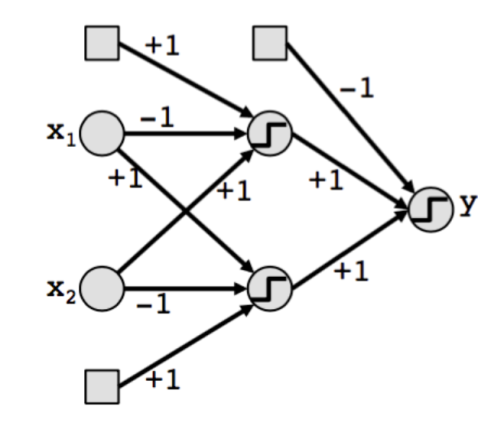
\includegraphics[width=0.5\textwidth]{Figures/BinaryConnect.png}
	\caption{Exemple d'un BinaryConnect à une seule couche cachée}
	\label{fig:BinaryConnect}
\end{figure}
\subsection{Topologie}
BinaryNet est indépendent de l'architecture choisie: Elle peut être dense, convolutionnelle, récurrente, etc\dots 
\newline Mais en pratique, il n'est testé que dans le cas dense et convolutionnel.



\subsection{Utilisation d'Estimateur Direct de gradient}
\subsubsection{Problématique}
Puisque la fonction signe est constante par morceau, son dérivé est donc nulle presque partout (dans le sens de la théorie des mesures).
\newline Ainsi, tout algorithme basé sur le gradient doit mettre en considération
\subsubsection{Principe}
L'entraînement d'un BNN est similaire à un RN classique:
\begin{enumerate}
	\item Une propagation en avant pour calculer la valeur de la fonction objective
	\item Une propagation en arrière pour calculer le gradient des paramètres
	\item La mise à jour des paramètres
	\item Refaire l'étape 1, jusqu'à satisfaire un critère bien déterminé (convergence, dépassement de la limite des époches, taux d'entraînement négligeable, etc...)
\end{enumerate}

L'estimateur direct de gradient\cite{STEPaper} sert à corriger le problème du gradient nul en faisant une estimation plus régulière de la fonction signe dans la propagation arrière (la fonction signe reste toujours utilisée dans la propagation avant)

L'estimation utilisée de la fonction $\sign$ est la fonction $\hardtanh$ définie par:
\begin{align*}
	\hardtanh:& \mathbb{R}\rightarrow \mathbb{R} \\
	&x\rightarrow \begin{cases}
		-1 & \text{si } x < -1 \\
		x & \text{si } \lvert x\rvert \leq 1 \\
		1 & \text{si }  x > 1
	\end{cases}
\end{align*}

En faite son dérivé est:
\begin{align*}
	\forall x \in\mathbb{R},\quad \dfrac{\partial \hardtanh}{\partial x}(x)&=\mathds{1}_{\lvert r \rvert \leq 1}(x)\\
	&=
	\begin{cases}
		1 & \text{si } \lvert x \rvert \leq 1 \\
		0 & \text{sinon}
	\end{cases}
\end{align*}

\begin{figure}[h!]
	\centering
	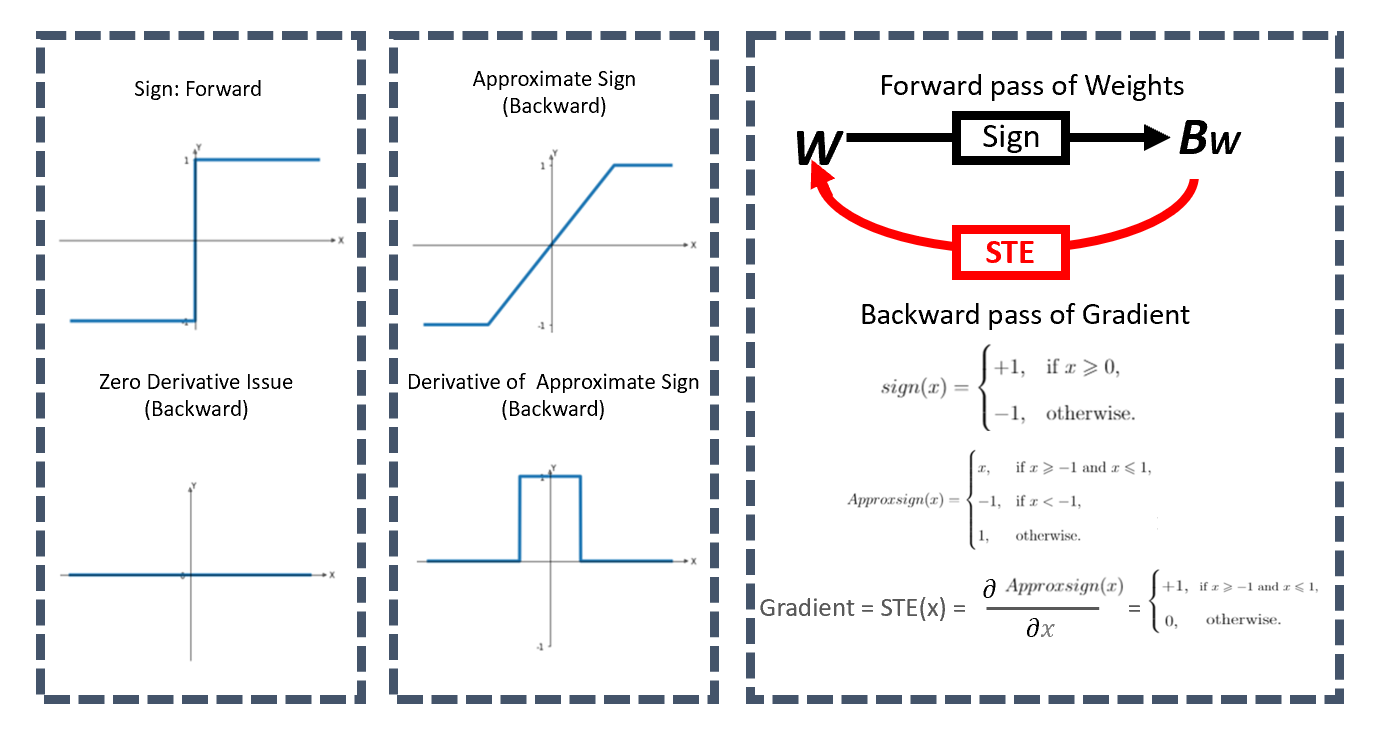
\includegraphics[width=1\textwidth]{Figures/STE.png}
	\caption{Estimateur direct du gradient}
	\label{fig:STE}
\end{figure}
\FloatBarrier

\subsubsection{Estimation du gradient}
Soit $f$ une fonction
Soit $\boldsymbol{x},\boldsymbol{y}$ deux tenseurs tels que $f(\bold{x})=y$ On note par $\mathcal{G}_{\boldsymbol{x}}$ l'estimation de gradient $\dfrac{\partial \mathcal{L}}{\partial \boldsymbol{x}}$ (par la méthode STE) et on la définit par:
$$
\mathcal{G}_{\boldsymbol{x}}=\begin{cases} 
	\dfrac{\partial \mathcal{L}}{\partial \boldsymbol{x}} \odot \mathds{1}_{\lvert \boldsymbol{x} \rvert \leq 1} & \text{si } f=\sign\\
	\mathcal{G}_y \cdot \dfrac{\partial \boldsymbol{y}}{\partial \boldsymbol{x}} & \text{sinon}
\end{cases}
$$

\begin{remark}
	Le calcul de $\mathds{1}_{\lvert \boldsymbol{x} \rvert \leq 1}$ se failt élément par élément. 
\end{remark}
\begin{remark}
	L'opérateur $\odot$ dénote la multiplication élément par élément
\end{remark}

La mise à jour des paramètres se fait en remplaçant chaque gradient par son estimation.

\subsubsection{Justification Théorique}
\subsection{Optimisations possible}
Etant un réseau totalement binarisé dans les couches cachées, BinaryConnect peut avoir plusieurs optimisations, y compris:
\begin{itemize}
	\item Utilisation du Codage binaire
	\item Utilisation des instructions $\mathtt{XNOR}$ est $\mathtt{POPCOUNT}$ pour accélerer la propagation avant
	\item Utilisation de ADA-Max pour accélérer la mise à jour des paramètres
	\item Utilisation de "Shifted Batch Normalisation" pour accélérer le calcul de la normalisation par lots.
\end{itemize}
\newpage

\section{XNOR-NET}
\subsection{Conception}
XNOR-NET\cite{XnorNetPaper} est le premier réseau de neurones binaires admettant des performances acceptables. Il est basé sur BinaryNet, et il met  l'accent sur l'utilisation de $\mathtt{XNOR}$ et $\mathtt{POPCOUNT}$ \cite{XnorNetPaper}.

De plus, Il introduit une nouvelle approche pour réduire l'erreur de quantification



\subsection{Topologie}
Comme BinaryConnect, XNOR-NET\cite{XnorNetPaper} est indépendent de l'architecture et la topologie utilisée.

En autre partie, il n'est pratiquement implémenté que dans les architectures denses et convolutionnelles.

\subsection{Réduction de l'erreur de quantification}
Pour $\boldsymbol{W}^{(l)}$ et $a^{(l-1)},$ on veut trouver deux facteurs $\alpha,\beta \in\mathbb{R}_+,$ et deux binarisations $\tilde{\boldsymbol{W}}^{(l)}$ et $\tilde{a}^{(l-1)}$ respectivement de $\boldsymbol{W}^{(l)}$ et $a^{(l-1)}$ tels que:
\begin{align}
	\boldsymbol{W}^{(l)} & \approx \alpha  \tilde{\boldsymbol{W}}^{(l)} \label{XnorNet:W}\\ 
	 \tilde{a}^{(l-1)} & \approx \beta  \tilde{a}^{(l-1)} \label{XnorNet:a}\\
	 \boldsymbol{W}^{(l)}\star a^{(l-1)} &\approx \alpha \beta  \tilde{\boldsymbol{W}}^{(l)}\star \tilde{a}^{(l-1)} \label{XnorNet:z}
\end{align}

Dans l'objectif décrit, les binarisations ne sont pas nécessairement la fonction $\sign,$ mais on montrera que c'est toujours un bon choix.
\subsection{Quantification optimale d'un vecteur}\label{XnorNet:VectorQuantification}
Dans cette section, nous allons trouvé les paramètres $\alpha$ et $\beta$ optimaux des équation respectifs \eqref{XnorNet:W} et \eqref{XnorNet:a} sans tenir compte de l'équation \eqref{XnorNet:z}.
\newline C'est à dire, nous allons dériver les quantification optimales de $\boldsymbol{W}^{(l)}$ et $a^{(l-1)}$ sans tenir compte de la qualité de la quantification \eqref{XnorNet:z} de $z^{(l)}=\boldsymbol{W}^{(l)}\star a^{(l-1)}.$
\newline En effet, nous allons raisonner d'une manière générale. Et puis les deux résultats vont être immédiatement déduits.

\subsubsection{Notations}
On va dénoter par:
\begin{itemize}
	\item $n\in\mathbb{N}^*$ la dimension de notre espace vectoriel.
	\item  $w$ un vecteur de $\mathbb{R}^n.$
	\item $\tilde{w}\in \{-1,1\}^n$ une binarisation de $w.$
	\item $\gamma\in\mathbb{R}_+$ un facteur d'échelle.
\end{itemize}
\subsubsection{Objectif}
L'objectif est de trouver $\tilde{w}$ et $\gamma$ qui minimisent $\lVert w-\gamma \tilde{w}\rVert_2^2$ pour un $u$ donné:
\begin{equation}\label{XnorNet:VectorQuantification:Problem}
	(\gamma,w)=\argmin_{\gamma,\tilde{w}}\lVert w-\alpha \tilde{w}\rVert_2^2
\end{equation} 
\subsubsection{Résolution du problème}
On a:
\begin{align*}
	\forall \gamma \in \mathbb{R},\forall \tilde w \in \{-1,1\}^n, \quad \lVert w - \gamma\tilde w \rVert_2^2 &= \langle w , w \rangle -2\gamma  \langle w , \tilde w\rangle + \gamma ^2\langle \tilde w , \tilde w \rangle   \\
	&=  \langle w , w \rangle -2\gamma \langle w , \tilde w\rangle + n\gamma ^2 \\
	\text{car }\tilde w \in\{-1,1\}^n,\quad \lVert \tilde w \rVert_2^2 &= \sum_{i=1}^n\tilde w_i^2 = n  
\end{align*}

Maintenant, on a $\langle w,\tilde w \rangle$ est maximisé pour $\tilde w=\sign w,$ et par conséquent puisque $\gamma \ge 0$
\newline $ \langle w , w \rangle -2\gamma \langle w , \tilde w\rangle + n\gamma ^2$ est minimisé pour $\tilde w=\sign w \quad \forall \gamma \in\mathbb{R}_+.$
\newline Ainsi le problème est réduit à la minimisation de la fonction quadratique suivante:
\begin{equation}
	H(\gamma)=\langle w , w \rangle -2\gamma \langle w , \sign w\rangle + n\gamma ^2
\end{equation}

En effet, $H$ étant une fonction convexe sur $\mathbb{R},$ admet un unique minimum local en $x^*=\frac{\langle w,\sign w\rangle}{n}.$
\newline Or, on a:
\begin{align*}
	x^*&=\frac{\langle w,\tilde w \rangle}{n}= \frac{1}{n}\sum_{i=1}^n w_i \sign w_i \\
	&= \frac{1}{n} \sum_{i=1}^n \lvert w_i\rvert = \frac{\lVert w \rVert_1}{n} \ge 0
\end{align*}
Ainsi, $\gamma = x^*$, et donc l'expression de $\gamma$ est:
\begin{equation}
	\gamma = \frac{\lVert w \rVert_1}{n}
\end{equation}

\subsubsection{Quantification de $\boldsymbol{W}^{(l)}$}
On a $\boldsymbol{W}^{(l)} \in E$ où $E\cong \mathbb{R}^{n_1}$ avec $n_1=\dim \boldsymbol{W}^{(l)}.$
\newline Ainsi, on a $\lVert \boldsymbol{W}^{(l)} - \alpha \tilde{\boldsymbol{W}}^{(l)} \rVert_2^2$ est minimisé pour:
\begin{equation}\label{Xnor:W:Expression}
	\begin{cases}
		\alpha &= \frac{\lVert \boldsymbol{W}^{(l)} \rVert }{n_1} \\ 
		\tilde{\boldsymbol{W}}^{(l)} &=\sign \boldsymbol{W}^{(l)}
	\end{cases}
\end{equation}
\subsubsection{Quantification de $a^{(l)}$}
On a $a^{(l)} \in F$ où $F\cong \mathbb{R}^{n_2}$ avec $n_2=\dim a^{(l)}.$
\newline Ainsi, on a $\lVert a^{(l)} - \beta \tilde{a}^{(l)} \rVert_2^2$ est minimisé pour:
\begin{equation}\label{Xnor:a:Expression}
	\begin{cases}
		\beta &= \frac{\lVert a^{(l)} \rVert }{n_2} \\ 
		\tilde{a}^{(l)} &=\sign a^{(l)}
	\end{cases}
\end{equation}

\subsection{Quantification d'un produit scalaire de deux vecteurs}\label{XnorNet:InnerProductQuantification}
Dans cette partie, nous allons tenir compte de la quantification de $z^{(l)},$ c'est à dire nous allons minimiser l'erreur de l'équation \eqref{XnorNet:z}.
\newline La résolution de cette équation n'est pas aussi triviale que \eqref{XnorNet:W}  et \eqref{XnorNet:a}, et donc nous allons majorer l'erreur de quantification $\lVert \langle  u,v \rangle - \langle  \alpha \tilde u,\beta \tilde v \rangle \rVert_2^2$ par une fonction plus facile à optimiser, et nous allons retrouver les expressions \eqref{Xnor:W:Expression} et \eqref{Xnor:a:Expression} de la section précédente.
\subsubsection{Objectif}
\begin{itemize}
\item Soit $n\in\mathbb{N}$ la dimension de l'espace euclidien.
\item Soit $u,v\in\mathbb{R}^n$  
\end{itemize}
Notre objectif est de trouver deux facteurs $\alpha,\beta \in\mathbb{R}_+$ et deux vecteurs $u,v\in\{-1,1\}^n$ qui réduisent $\lVert \langle  u,v \rangle - \langle  \alpha \tilde u,\beta \tilde v \rangle \rVert_2^2$
\subsubsection{Une Borne supérieure de l'erreur}
Une formule exacte pour le problème originale est un peu difficile. Pour cela, on pose $w=u\odot v,$ et on cherche une borne supérieure de $\lVert \langle  u,v \rangle - \langle  \alpha \tilde u,\beta \tilde v \rangle \rVert_2^2$ en fonction de $\lVert w-\alpha\beta \tilde u \odot \tilde v\rVert_2^2$ \cite{XnorNetPaper}:
\begin{align*}
	\lVert \langle  u,v \rangle - \langle  \alpha \tilde u,\beta \tilde v \rangle \rVert_2^2&=(\langle  u,v \rangle - \langle  \alpha \tilde u,\beta \tilde v \rangle)^2 \\
	&= \left(\sum_{i=1}^n u_iv_i-\alpha\beta \tilde u_i \tilde v_i\right)^2 \\
	&= \left\lvert \sum_{i=1}^n\sum_{j=1}^n (u_iv_i-\alpha\beta \tilde u_i\tilde v_i) (u_jv_j-\alpha\beta \tilde u_j\tilde v_j)  \right\rvert \\
	&\leq \sum_{i=1}^n\sum_{j=1}^n \lvert u_iv_i-\alpha\beta \tilde u_i\tilde v_i \rvert  \lvert u_jv_j-\alpha\beta \tilde u_j\tilde v_j \rvert \\
	&\leq \sum_{i=1}^n\sum_{j=1}^n \lVert u\odot v - (\alpha \tilde u) \odot (\beta \tilde v) \rVert_\infty^2\\
	&\leq n^2 \lVert u\odot v - (\alpha \tilde u) \odot (\beta \tilde v) \rVert_\infty^2\\
	&\leq n^2\lVert u\odot v - (\alpha \tilde u) \odot (\beta \tilde v) \rVert_2^2\\
	&\leq  n^2\lVert w - \alpha \beta \tilde u \odot \tilde v \rVert_2^2
\end{align*}

Avec ce résultat, on est sûr qu'en minimisant $\lVert w - \alpha \beta \tilde u \odot \tilde v \rVert_2^2,$ on minimise la borne supérieure de l'erreur de quantification.
\subsubsection{Minimisation de $\lVert w - \alpha \beta \tilde u \odot \tilde v \rVert_2^2$}
En effet, Puisque $\tilde u \odot \tilde v$ génère tout les vecteurs binaires, et $\alpha \beta$ génère tous les réels positifs, on peut trouver $\argmin\limits_{\alpha,\beta,\tilde u ,\tilde v} \lVert w - \alpha \beta \tilde u \odot \tilde v \rVert_2^2$ à partir de $\argmin\limits_{\gamma,\tilde w }\lVert w - \gamma\tilde w \rVert_2^2.$
\newline Or, on a déjà trouvé ce dernier. Ainsi on a:
\begin{equation}
	\begin{cases}
		\tilde u \odot \tilde v = \tilde w=\sign w = \sign u \odot \sign v \\
		\alpha\beta = \gamma = \frac{\lVert w \rVert_1}{n}
	\end{cases}
\end{equation}
\subsubsection{Valeur de $\alpha,\beta,\tilde{u}$ et $\tilde{v}$} 
Pour trouver chacune de $\alpha,\beta$ on fait les hypothèses suivantes:
\begin{itemize}
	\item $u_1,\dots,u_n$ et $\boldsymbol{x}$ suivent une distribution $\mathcal{U}$ à moment absolu de premier ordre fini. 
	\item $v_1,\dots,v_n$ et $\boldsymbol{y}$ suivent une distribution $\mathcal{V}$ à moment absolu de premier ordre fini.
	\item $\forall i,j\in\{1,\dots,n\},\quad u_i \text{ et } v_j \text{ sont indépendents}$ 
	\item $\alpha$ et $\tilde{u}$ ne dépendent que de $u$
	\item $\beta$ et $\tilde{v}$ ne dépend que de $v$
\end{itemize}

En exploitant les hypotèses proposées, on peut facilement trouver $\tilde{u}$ et $\tilde{v}$:
\begin{equation}\label{XnorNet:InnerProductQuantification:Binarisatiosn}
	\begin{cases}
		\tilde{u} = \sign u\\
		\tilde{v} = \sign v
	\end{cases}
\end{equation}
Pour $\alpha$ et $\beta,$ on donne la démonstration suivante:
\begin{align*}
	\mathbb{E}[\gamma] &= \mathbb{E}\left[\frac{\lVert w \rVert_1}{n}\right] = \frac{1}{n}\mathbb{E}\left[\lVert  w \rVert_1\right] \\
	&= \frac{1}{n}\sum_{i=1}^n\mathbb{E}\left[\lvert  u_i v_j \rvert\right] = \frac{1}{n}\sum_{i=1}^n \mathbb{E}\left[\lvert  u_i \rvert]\mathbb{E}[\lvert  v_j \rvert\right] \\
	&= \frac{1}{n}\sum_{i=1}^n \mathbb{E}\left[\lvert  \boldsymbol{x} \rvert\right]\mathbb{E}\left[\lvert \boldsymbol{y} \rvert\right] = \mathbb{E}\left[\lvert  \boldsymbol{x} \rvert\right]\mathbb{E}\left[\lvert \boldsymbol{y} \rvert\right]\\
	&= \mathbb{E}\left[\frac{\lVert u \rVert_1}{n}\right] \times \mathbb{E}\left[\frac{\lVert v \rVert_1}{n}\right]\\
	&= \mathbb{E}\left[\alpha \right]\mathbb{E}\left[\beta \right]
\end{align*}  
Ainsi avec les hypothèses proposées on trouve $\mathbb{E}\left[\alpha \right]=\mathbb{E}\left[\lvert  \boldsymbol{u} \rvert\right]$ et $\mathbb{E}\left[\beta \right]=\mathbb{E}\left[\lvert  \boldsymbol{v} \rvert\right],$ et donc: 
\begin{equation} \label{XnorNet:InnerProductQuantification:ScaleFactors}
	\begin{cases}
		\alpha \approx \frac{\lVert u \rVert_1}{n}\\
		\beta \approx \frac{\lVert v \rVert_1}{n}
	\end{cases}
\end{equation}
\newline En conclusion, on trouve\cite{XnorNetPaper}:
\begin{equation} \label{XnorNet:InnerProductQuantification:Result}
	\begin{cases}
		u \approx \frac{\lVert u \rVert_1}{n}\sign u \\
		v \approx \frac{\lVert v \rVert_1}{n}\sign v
	\end{cases}
\end{equation}

\subsection{Quantification d'une couche dense par produits scalaires}
Dans ce cas, on a:
\begin{equation*}
	\boldsymbol{W}^{(l)}a^{(l-1)} = \begin{pmatrix}
		\langle \boldsymbol{W}_1^{(l)}, a^{(l-1)} \rangle  \\
		\vdots  \\
		\langle \boldsymbol{W}_{n_l}^{(l)}, a^{(l-1)} \rangle 
	\end{pmatrix}
\end{equation*}
On applique la réduction d'erreur de quantification élément par élément:
\begin{equation}
	\begin{cases}
		a^{(l-1)} \approx \beta \sign a^{(l-1)} & \beta = \frac{\lVert a^{(l-1)}\rVert_1}{n_{l-1}} \\ 
		\forall i\in\{1,\dots,n_l\},\quad \boldsymbol{W}_i^{(l)} \approx \alpha_i \sign \boldsymbol{W}_i^{(l)} & \alpha_i = \frac{\lVert \boldsymbol{W}_i^{(l)} \rVert_1 }{n_{l-1}}
	\end{cases}
\end{equation}

Ainsi 
\begin{align*}
	\boldsymbol{W}^{(l)}a^{(l-1)} &\approx  \begin{pmatrix}
		\beta \alpha_1 \langle \sign \boldsymbol{W}_1^{(l)}, \sign a^{(l-1)} \rangle  \\
		\vdots  \\
		\beta \alpha_{n_l} \langle \sign \boldsymbol{W}_{n_l}^{(l)}, \sign a^{(l-1)} \rangle 
	\end{pmatrix} \\ 
	&\approx \beta  \left(\sign \boldsymbol{W}^{(l)} \sign a^{(l-1)}\right) \odot \boldsymbol{\alpha}  \addtocounter{equation}{1}\tag{\theequation} \label{XnorNet:FullyConnected}
\end{align*}

\begin{figure}[h!]
	\centering
	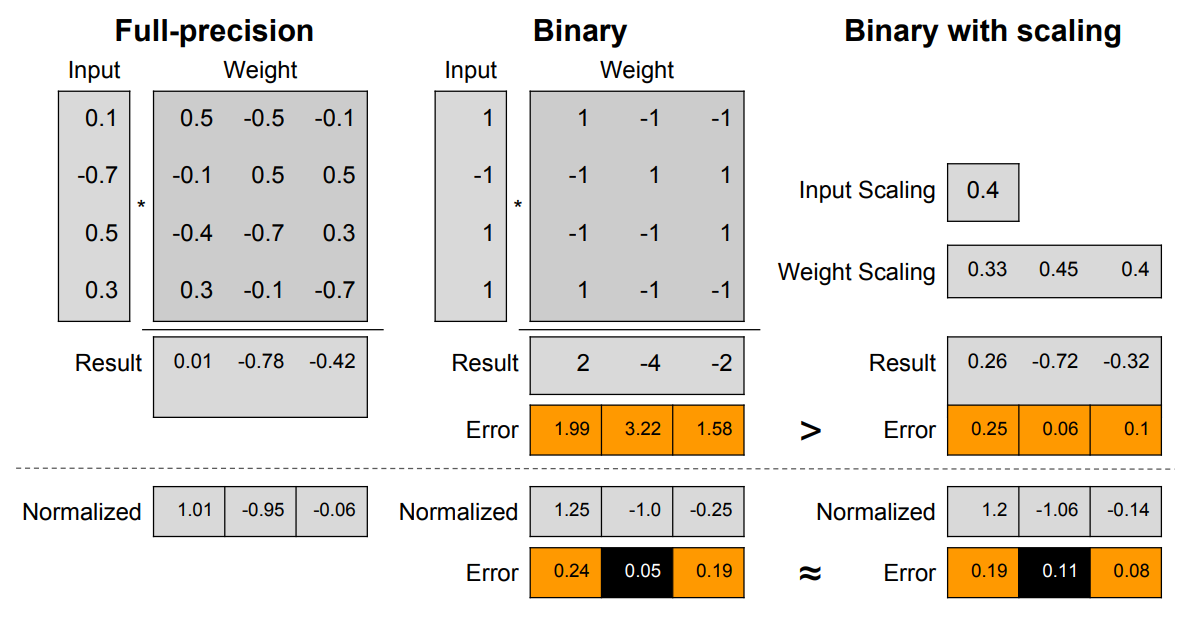
\includegraphics[width=1\textwidth]{Figures/XNOR-Scaling.png}
	\caption{Utilisation de facteurs $\alpha$ et $\beta$ dans une couche denseUtilisation de facteurs $\alpha$ et $\beta$ dans une couche dense}
	\label{fig:XNOR-Dense}
\end{figure}
\FloatBarrier

\subsection{Quantification d'une couche convolutionnelle par produits scalaires }
\begin{remark}
	Nous allons raisonner sur les convolutions à $2$ dimensions. Mais en effet, les résultats peuvent être trivialement généralisés.
\end{remark}
\begin{remark}
	Pour trouver des expressions de $\alpha$ et $\beta,$ nous allons raisonner sur une convolution sans strides ni dilation, ni groupements. On va proposer ensuite un truc qui permet de recouvrer les formules de $\alpha$ et $\beta$ dans ces cas. 
\end{remark}
Soit $\boldsymbol{W}^{(l)}$ une couche convolutionnelle qui prends $C_{\text{in}}$ canaux et donne $C_{\text{out}}$ canaux et dont les noyaux sont de dimensions $(w,h)$.

La formule de $z^{(l)}$ est:
\begin{equation}\label{eq:ConvExpanded}
	\forall c\in\{1,\dots, C_{\text{out}}\},\quad z_c^{(l)}=\sum_{c'=1}^{C_\text{in}} \boldsymbol{W}_{c,c'}^{(l)}*a_{c'}^{(l-1)}
\end{equation}

\begin{remark}
	On peut aussi écrire \eqref{eq:ConvExpanded} sous la forme compacte:
	\begin{equation}
	z^{(l)}= \boldsymbol{W}^{(l)}* a^{(l-1)}
	\end{equation}
	où $\boldsymbol{W}^{(l)}$ est de dimension $C_{\text{out}}\times C_{\text{in}} \times w\times h,$ et $a^{(l-1)}$ est de dimension  $C_\text{in}\times w \times h$
\end{remark}
Pour simplifier, nous allons raisonner sur le cas $C_{\text{out}}=1,$ puis nous allons généraliser:
\subsubsection{Cas d'un seul canal de sortie: $C_{\text{out}}=1$}
On commence par le cas $C_{\text{out}}=1:$
On a:
\begin{align}
	\alpha&=\frac{\left\lVert \boldsymbol{W}^{(l)} \right\rVert_1}{w\cdot h \cdot C_{\text{in}}} \\
	\forall i,j\quad \beta_{i,j}&=\frac{\left\lVert a_{[i,w],[j,h]}^{(l-1)} \right\rVert_1}{w\cdot h \cdot C_{\text{in}} }
\end{align}
avec $a^{(l-1)}_{[i,w],[j,h]}$ est le sous-tenseur de dimensions $C_{\text{in}} \times w \times h$ qui commence à la position $i$ dans son deuxième axe, et $j$ dans son troisième axe.

En faite, $(\beta_{i,j})_{i,j}$ constitue un tenseur $\boldsymbol{\beta}$\footnote{Le temps de calcul de $\boldsymbol{\beta}$ peut être optimisé grâce aux techniques de la programmation dynamique} de dimension $w\times h,$ et la formule de $z^{(l)}$ sera:
\begin{equation} \label{XnorNet:Conv}
	z^{(l)}=\left(\sign \boldsymbol{W}^{(l)} * \sign a^{(l-1)}\right) \odot \boldsymbol{\beta}\alpha
\end{equation}

\subsubsection{Cas général}
Dans le cas où $C_{\text{out}}>1$, on décompose cette couche convolutionnelle en plusieurs convolutions. et on dérive la formule de chacune:
\begin{equation}
	\forall c\in\{1,\dots, C_{\text{out}\}},\quad z_c^{(l)} = \left(\sign \boldsymbol{W}_c^{(l)} * \sign a^{(l-1)}\right) \odot \boldsymbol{\beta}\alpha_c
\end{equation}
Finalement, on peut l'écrire dans la forme compacte:
\begin{equation}
	z^{(l)} = \left(\sign \boldsymbol{W}^{(l)} * \sign a^{(l-1)}\right) \odot \left(\boldsymbol{\alpha} \otimes \boldsymbol{\beta}\right)
\end{equation}
où $\otimes$ est le produit extérieur entre deux tenseurs.

\begin{figure}[h!]
	\centering
	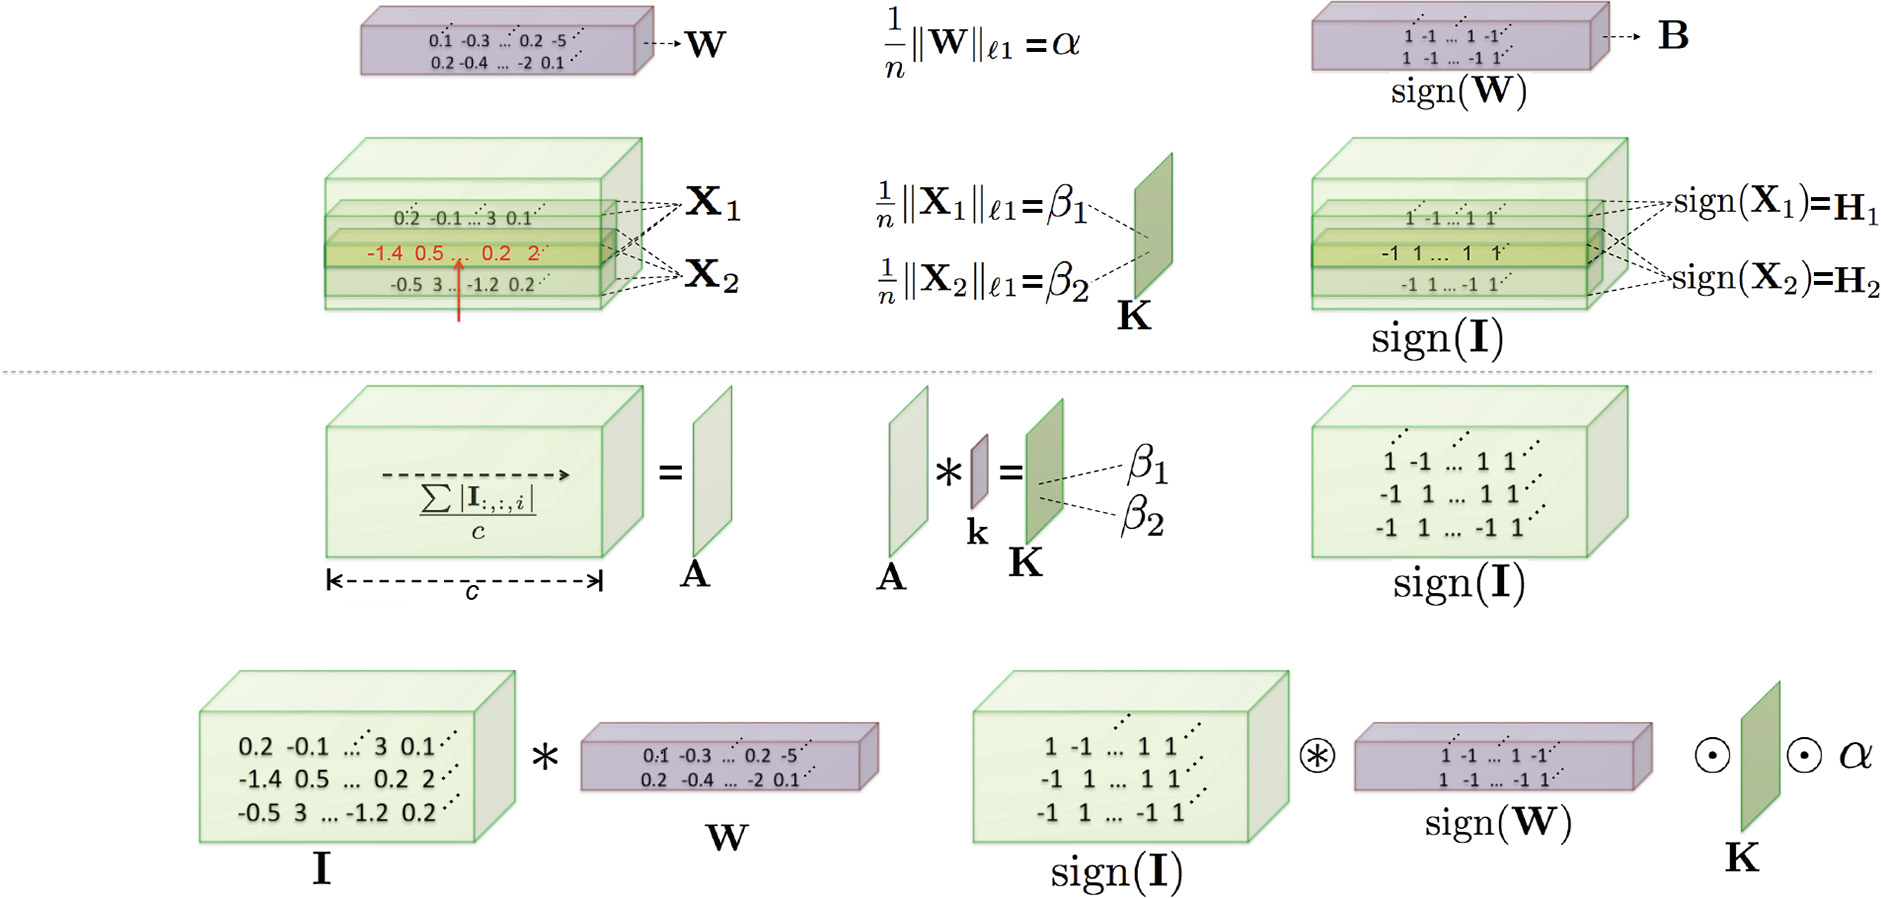
\includegraphics[width=1\textwidth]{Figures/XNOR-Conv2D.png}
	\caption{Utilisation de facteurs $\alpha$ et $\beta$ dans une couche convolutionnelle}
	\label{fig:XNOR-Conv}
\end{figure}
\FloatBarrier
\subsection{Quantification d'une opération bilinéaire quelconque}\label{XnorNet:BilinearForm}
\subsubsection{Hypothèses}
Les hypothèses suivantes ne posent aucune contrainte supplémentaires, en effet on les pose pour formaliser notre démonstration:
\begin{itemize}
\item On suppose que $\boldsymbol{W}^{(l)}$ et $a^{(l-1)}$ sont deux membres des espaces vectoriels réels respectifs $E_l$ et $F_{l-1}.$
\item On suppose que $\star : E_l\times F_{l-1}\rightarrow H_l$ est bilinéaire avec $H_l$ est un espace vectoriel réel de dimension $\dim H_l=s$.
\item On suppose que $\mathcal{B}_1$ et $\mathcal{B}_2$ sont les bases respectifs de  $E_l$ et $F_{l-1}.$
\end{itemize}
\subsubsection{Décomposition de $\star$ en formes bilinéaires}
On a $\star$ peut être décomposé élément par élément en $s$ forme bilinéaire $\star_1,\dots,\star_s:E_l\times F_{l-1} \rightarrow \mathbb{R}.$
\newline Soit $M_i=\mat(\star_i,\mathcal{B}_1,\mathcal{B}_2).$ On a donc:
\begin{equation*}
	\boldsymbol{W}^{(l)}\star a^{(l-1)} = \begin{pmatrix}
	\boldsymbol{W}^{(l)}\star_1 a^{(l-1)}	 \\
	\vdots \\
	\boldsymbol{W}^{(l)}\star_s a^{(l-1)}
		\end{pmatrix} =
	\begin{pmatrix}
		{\boldsymbol{W}^{(l)}}^T M_1 a^{(l-1)}	\\
		\vdots \\
		{\boldsymbol{W}^{(l)}}^T M_s  a^{(l-1)}
	\end{pmatrix} 
\end{equation*}
\subsubsection{Décomposition en valeurs singulières}
Dans cette section, nous allons quantifier chaque forme bilinéaire indépendamment de l'autre.
\newline Soit $i\in\{1,\dots,s\}.$  On a d'après la décomposition en valeurs singulières:
\begin{equation*}
	\exists V_i\in \mathcal{O}(\mathbb{R},m),\exists U_i\in\mathcal{O}(\mathbb{R},n),\exists \Sigma_i\in\mathcal{M}(\mathbb{R},n,m) \ \text{diagonal}\ / \quad \begin{cases}
		M_i= U_i^T \Sigma_i V_i \\ 
		\Sigma_{i,p,p}=\sigma_{i,p} \ge 0 & \forall p\in\{1,\dots,\min(n,m)\} \\
		\Sigma_{i,p,p}=\sigma_{i,p} = 0 & \forall p> \min(n,m)
	\end{cases}
\end{equation*}
On peut encore factoriser $\Sigma_i$ en deux matrices diagonales $A_i\in\mathcal{M}(\mathbb{R},\min(n,m),n)$ et $B_i \in\mathcal{M}(\mathbb{R},\min(n,m),m)$ tels que:
\begin{equation}
	\begin{cases}
	A_{i,p,p}=B_{i,p,p} = \sqrt{\sigma_{i,p}}  &  \forall p \in\{1,\dots,\min(n,m)\} \\
	\Sigma_i = A_i^TB_i
	\end{cases}
\end{equation}
On a donc: 
\begin{align*}
	\boldsymbol{W}^{(l)}\star_i a^{(l-1)} &= {\boldsymbol{W}^{(l)}}^T M_i a^{(l-1)} \\
	&= {\boldsymbol{W}^{(l)}}^T U_i^T A_i^T B_i V a^{(l-1)} \\
	&=\left(A_iU_i \boldsymbol{W}^{(l)}  \right)^T \left(B_i V_i a^{(l-1)}\right) \\
	&= \left\langle A_iU_i \boldsymbol{W}^{(l)}  , B_i V_i a^{(l-1)}  \right\rangle  \addtocounter{equation}{1}\tag{\theequation}
\end{align*}
Pour quantifier ce produit scalaire, on doit d'abord généraliser l'équation \eqref{XnorNet:VectorQuantification:Problem} en:

\begin{equation}\label{XnorNet:TransformedVectorQuantification}
	(\gamma,\tilde{w})=\argmin_{\gamma,\tilde{w}} \lVert A U w -  \gamma A U \tilde{w} \rVert_2^2
\end{equation}
Avec \begin{itemize}
	\item $A\in\mathcal{M}(\mathbb{R},m,n)$ une matrice diagonale dont les coefficient diagonaux $A_{p,p}=\sqrt{\sigma_p}$ sont positifs
	\item $U\in\mathcal{O}(\mathbb{R},n)$ une matrice orthogonale. 
\end{itemize}
\subsubsection{Quantification optimale de $A U w$ }
Avant de résoudre ce problème, nous allons utilisé la propriété suivante:
\begin{equation} \label{SVD:Lemma1}
	U^TA^TA U = A^TA = D ^2
\end{equation}
Avec $D \in\mathcal{M}(\mathbb{R},m)$ la matrice diagonale tels que $D_{p,p}=\sqrt{\sigma_p}$
\newline En effet, en exploitant \eqref{SVD:Lemma1} on a:
\begin{align*}
	\lVert A U w -  \gamma A U \tilde{w} \rVert_2^2 &= \langle A U w,A U w \rangle - 2\gamma \langle A U w, A U \tilde{w} \rangle + \gamma ^2\langle A U \tilde{w},A U \tilde{w} \rangle \\
	&= \langle A U w,A U w \rangle - 2\gamma \langle A U w, A U \tilde{w} \rangle + \gamma ^2\langle A U \tilde{w},A U \tilde{w} \rangle \\
	&= \langle  w,U^TA ^T A U w \rangle - 2\gamma \langle  w, U^TA ^TA U \tilde{w} \rangle + \gamma ^2\langle  \tilde{w},U^TA^T A U \tilde{w} \rangle \\
	&= \langle  w,D^2  w \rangle - 2\gamma \langle  w, D^2 \tilde{w} \rangle + \gamma ^2\langle  \tilde{w},D^2 \tilde{w} \rangle  \\
	&=\langle  D w,D  w \rangle - 2\gamma \langle  D w, D \tilde{w} \rangle + \gamma ^2\langle  D \tilde{w},D \tilde{w} \rangle
\end{align*}
Or on a:
\begin{equation*}
	\langle  D\tilde{w},D \tilde{w} \rangle  = \sum_{i=1}^n \sigma_i \tilde{w}_i^2 = \sum_{i=1}^n \sigma_i
\end{equation*}
Et donc on a:
\begin{equation*}
	\left\lVert \Sigma V w -  \gamma \Sigma V \tilde{w} \right\rVert_2^2 =  \langle  D w,D  w \rangle - 2\gamma \langle  D w, D \tilde{w} \rangle + \gamma ^2\sum_{i=1}^n \sigma_i
\end{equation*}
Maintenant, d'une façon analogue à la démonstration de \ref{XnorNet:VectorQuantification}, on peut montrer que $\langle D w,D \tilde{w} \rangle$ est maximisé pour $\tilde{w} = \sign w$, et donc puisque $\gamma \ge 0,$ on a $	\lVert A U w -  \gamma A U \tilde{w} \rVert_2^2$ est minimisé pour $\tilde{w}=\sign w$ indépendamment de $\gamma.$
\newline En s'inspirant de \ref{XnorNet:VectorQuantification}, on trouve:
\begin{equation} \label{XnorNet:TransformetVectorQuantification:Result}
	\begin{cases}
		\gamma &= \dfrac{\sum_{i=1}^n \sigma_i \lvert w_i \rvert }{\sum_{i=1}^n \sigma_i}\\
		\tilde{w} &= \sign w 
	\end{cases}
\end{equation}
\subsubsection{Quantification optimale de $A_i U_i \boldsymbol{W}^{(l)}$ }
D'après la résolution du problème \eqref{XnorNet:TransformedVectorQuantification}, et en exploitant le résultat \eqref{XnorNet:TransformetVectorQuantification:Result}:
\begin{equation}
	\forall i \in\{1,\dots,r\}	\begin{cases}
		\alpha_i &= \dfrac{\sum_{j=1}^n \sigma_{i,j}\left\lvert \boldsymbol{W}^{(l)}_j \right\rvert }{\sum_{j=1}^n \sigma_{i,j}}\\
		\tilde{\boldsymbol{W}}^{(l)} &= \sign \boldsymbol{W}^{(l)}
	\end{cases}
\end{equation}
\subsubsection{Quantification optimale de $B_i V_i a^{(l-1)}$ }
De même, on trouve que:
\begin{equation}
\forall i \in\{1,\dots,s\}	\begin{cases}
		\beta_i &= \dfrac{\sum_{j=1}^n \sigma_{i,j} \left\lvert a^{(l-1)}_j \right\rvert }{\sum_{j=1}^n \sigma_{i,j}}\\
		\tilde{a}^{(l-1)} &= \sign a^{(l-1)}
	\end{cases}
\end{equation}

\subsubsection{Quantification de l'opérateur bilinéaire}
Le résultat final est peut être écrit sous cette forme compacte:
\begin{equation}\label{XnorNet:BilnearForm:Result}
	\boldsymbol{W}^{(l)}\star a^{(l-1)} \approx  \left( \sign \boldsymbol{W}^{(l)} \star \sign a^{(l-1)}\right) \odot \boldsymbol{\alpha} \odot \boldsymbol{\beta}
\end{equation}

\pagebreak
\section{ABCNet}
\subsection{Conception}
ABCNet\cite{ABCNetPaper} est un réseau de neurones binaires basé sur XNOR-Net, son nom est une abbréviation de "Accurate Binary Convolutional Network", et donc comme son nom suggeste, il est très performant (comparable à un CNN classique). 
\newline Il peut être considéré comme une amélioration directe de XnorNet, puisqu'il réduit l'erreur de quantification d'une variable en faisant une somme pondérée de binarisations prédéfinie.
\begin{figure}[h!]
	\centering
	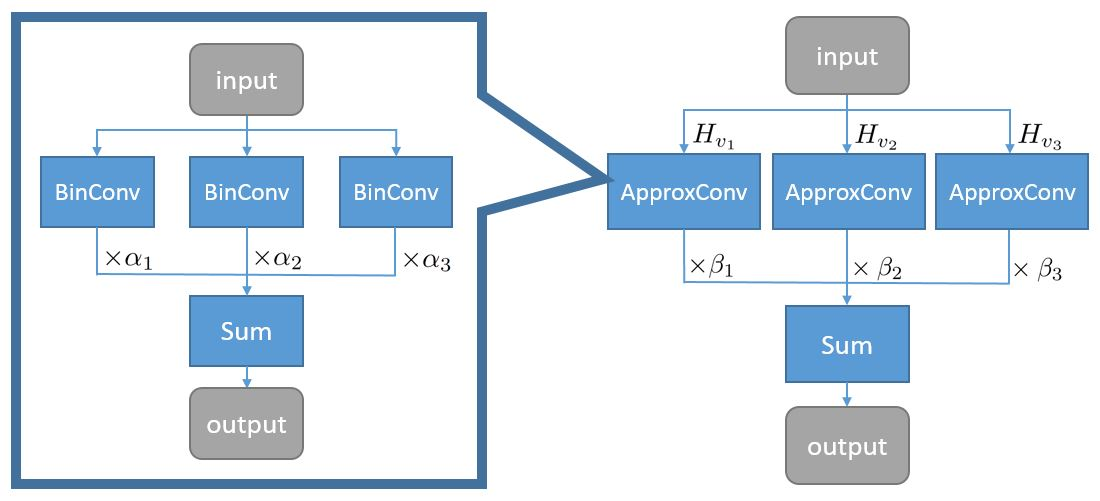
\includegraphics[width=\textwidth]{Figures/ABCNet.png}
	\caption{Exemple d'un ABCNet à une seule couche}
	\label{fig:ABCNet}
\end{figure}
\subsection{Toplogie}
Le ABCNet\cite{ABCNetPaper} est conçu explicitement pour les réseaux de neurones binaires convolutionnelles. 

Mais comme le XNOR-NET, il peut être généralisé à n'importe quel architecture (dense, récurrente, etc...)
\subsection{Objectif}
\subsubsection{Notations}
On dénote par
\begin{enumerate}
	\item $\Psi_1,\dots,\Psi_n$ des binarisations de  $\boldsymbol{W}^{(l)}$
	\item $\Phi_1,\dots,\Phi_m$ des binarisations de  $a^{(l-1)}$
\end{enumerate}
\subsubsection{Approximation par combinaisons linéaires}
L'objectif d'un ABCNet est d'approximer $\boldsymbol{W}^{(l)}$ en une combinaison linéaires de $n$ binarisations, et $a^{(l-1)}$ en $m$ une combinaison linéaires de $m$ binarisations.

On veut trouver $\left(\Psi_1,\dots,\Psi_n\right), \left(\Phi_1,\dots,\Phi_m\right),(\alpha_1,\dots,\alpha_n)\in\mathbb{R}_+^n,(\beta_1,\dots,\beta_m)\in\mathbb{R}_+^m $ tel que:
\begin{align}
	\boldsymbol{W}^{(l)}&\approx \sum_{i=1}^n \alpha_i \Psi_i(\boldsymbol{W}^{(l)}) \label{ABCNet:W}  \\
	a^{(l-1)}&\approx \sum_{i=1}^m \beta_i \Phi_i(a^{(l-1)}) \label{ABCNet:a}\\
	\boldsymbol{W}^{(l)} \star a^{(l-1)} &\approx \sum_{i=1}^n\sum_{j=1}^m  \alpha_i  \beta_j\Psi_i(\boldsymbol{W}^{(l)})\star  \Phi_j(a^{(l-1)}) \label{ABCNet:z}
\end{align}

\subsection{Choix de binarisations de $\boldsymbol{W}^{(l)}$}
Il y'a plusieurs méthodes pour choisir les binarisations de $\boldsymbol{W}^{(l)}$
\subsubsection{Base orthogonale de Hadamard}
Cette technique crée des binarisations qui ne dépendent pas de $\boldsymbol{W}^{(l)}.$ En interprétant $\boldsymbol{W}^{(l)}$ comme un vecteur d'un espace euclidien $E$ de dimension $r=2^s\ge n.$ On  cherche la matrice de Hadamard $H_s,$ puis on choisit $n$ colonnes (ou lignes) $\Psi_1,\dots,\Psi_n$.

Dans ce cas, la famille $(\Psi_1,\dots,\Psi_n)$ induit un sous-espace $F$ de $E$ de dimension $n.$  
\newline Ainsi, le problème est réduit à une projection orthogonale de $E$ vers $F$    
\newline En notant $K=\mat(\Psi_1,\dots,\Psi_n),$ la valeur optimale de $\boldsymbol{\alpha}$ qui minimise l'erreur quadratique de quantification est:
\begin{equation}
	\boldsymbol{\alpha} = K^T\boldsymbol{W}^{(l)}
\end{equation}

\subsubsection{Famille de fonctions $\sign$ décalées } 
Cette technique crée des binarisations de la forme:
\begin{equation}
	\Psi_i\left(\boldsymbol{W}^{(l)}\right) = \sign \left( \boldsymbol{W}^{(l)} +\mu_i\right) 
\end{equation}
Avec $\mu_1,\dots,\mu_n\in\mathbb{R}$ un paramètre de décalage. Il peut être entraînable ou non.

\subsubsection{Approximation par distribution}
Cette technique se base sur l'observation que la distribution des poids (non-binarisés) est dense\cite{ABCNetPaper}, et elle est proche d'une distribution normale. L'expression de $\Psi_i$ est:
\begin{equation}
	\Psi_i\left(\boldsymbol{W}^{(l)}\right)=\sign\left( \boldsymbol{W}^{(l)}-\mathbb{E}\left[ \boldsymbol{W}^{(l)} \right] + \mu_i \sqrt{\mathbb{V}\left[ \boldsymbol{W}^{(l)} \right]}\right)
\end{equation}
Où \begin{itemize}
	\item $\mathbb{E}\left[ \boldsymbol{W}^{(l)} \right]$ est un estimateur de l'espérence de la distribution des paramètres: c'est la valeur moyenne de tous ces paramètres.
	\item  $\mathbb{V}\left[ \boldsymbol{W}^{(l)} \right]$ est une estimation de leur variance.
	\item $\mu_i$ est fixe ou entraînable.
\end{itemize}
Quelque soit le cas, on peut initialiser $\mu_i$\cite{ABCNetPaper} par:
\begin{equation}
	\mu_i=-1+2\cdot \frac{i-1}{n-1}
\end{equation}

\subsection{Choix de binarisations de $a^{(l)}$}
Puisque $a^{(l)}$ dépend toujours de l'entrée $x.$ Pour cela $a^{(l)}$ va généralement varier d'une inférence à une autre.
\newline Pour cela, on doit créer des binarisations qui dépendent de $a^{(l)}.$ Par exemple, on peut choisir:
\subsubsection{Famille de fonctions $\sign$ décalées}
Cette technique crée des binarisations de la forme:
\begin{equation}
	\Psi_j\left(a^{(l)}\right) = \sign \left( a^{(l)} +\kappa_j\right) 
\end{equation}
Avec $\kappa_1,\dots,\kappa_m\in\mathbb{R}$ un paramètre de décalage. Il peut être entraînable ou non.

\subsubsection{Approximation par distribution}
\begin{equation}
	\Phi_j\left(a^{(l)}\right)=\sign\left( a^{(l)}-\mathbb{E}\left[a^{(l)} \right] + \kappa_j \sqrt{\mathbb{V}\left[ a^{(l)} \right]}\right)
\end{equation}
Où \begin{itemize}
	\item $\mathbb{E}\left[ a^{(l)} \right]$ est une estimation de l'espérence de $a^{(l)}$ dans le lot courant.
	\item  $\mathbb{V}\left[a^{(l)} \right]$ est une estimation de la variance de $a^{(l)}$ dans le lot courant
	\item $\kappa_j$ est fixe ou entraînable.
\end{itemize}

Dans la phase d'inférence, pour éviter le côut de calcul des paramètres statistiques, on peut remplacer:
\begin{itemize}
	\item $\mathbb{E}\left[ a^{(l)} \right]$ du lot courant par $K_1=\mathbb{E}_B\left[\mathbb{E}\left[ a^{(l)} \right]\right],$ qui est la valeur moyenne de tous les lots du jeu de données.
	\item $\mathbb{V}\left[ a^{(l)} \right]$ du lot courant par $K_2=\frac{m}{m-1}\mathbb{E}_B\left[\mathbb{V}\left[a^{(l)} \right]\right]$, qui est une estimation sans bias de la variance de $a^{(l)}$ dans tous les lots du jeu de données, avec $m$ la taille de lot.
\end{itemize}

\subsection{Quantification par tenseur binaire}
C'est la méthode ou on fait les quantifications de $\boldsymbol{W}^{(l)}$ et $a^{(l-1)}$ en suivant les équations respectifs \eqref{ABCNet:W} et \eqref{ABCNet:a}
\newline La quantification de $z^{(l)}$ va respecter l'équation $\eqref{ABCNet:z}.$

\subsection{Quantification par produit scalaire}
La quantification par produit scalaire est une variante dans laquelle les variables $\alpha_1,\dots,\alpha_n$ de \eqref{ABCNet:W} et $\beta_1,\dots,\beta_m$ de \eqref{ABCNet:a} sont calculéss pour chaque produit scalaire.
\newline C'est à dire, L'équation $\eqref{ABCNet:z}$ est décomposée terme par terme en des produits scalaires, dans chacune on cherche les $(\alpha_i)_{i\in\{1,\dots,j\}}$ et $(\beta_j)_{j\in\{1,\dots,m\}}.$
\subsubsection{Couche Dense}
C'est une généralisation de l'équation \eqref{XnorNet:FullyConnected} de XnorNet.
\newline On a:
\begin{align*}
	\boldsymbol{W}^{(l)}\cdot a^{(l-1)} &\approx  \begin{pmatrix}
		 \left\langle \sum_{i=1}^n \alpha_{i,1}\Psi_i \left(\boldsymbol{W}_1^{(l)}\right),\sum_{j=1}^m \beta_j\Phi_j \left( a^{(l-1)}\right) \right\rangle  \\
		\vdots  \\
		\left\langle \sum_{i=1}^n \alpha_{i,n_l}\Psi_i \left(\boldsymbol{W}_{n_l}^{(l)}\right),\sum_{j=1}^m  \beta_j\Phi_j\left( a^{(l-1)}\right) \right\rangle 
	\end{pmatrix} \\
	&\approx  \begin{pmatrix}
		 \sum_{i=1}^n \sum_{j=1}^m \left \langle \alpha_{i,1}  \Psi_i \left(\boldsymbol{W}_1^{(l)}\right), \beta_j \Phi_j \left( a^{(l-1)}\right) \right\rangle  \\
		\vdots  \\
		\sum_{i=1}^n \sum_{j=1}^m \left \langle \alpha_{i,n_l}  \Psi_i \left(\boldsymbol{W}_{n_l}^{(l)}\right), \beta_j \Phi_j \left( a^{(l-1)}\right) \right\rangle 
	\end{pmatrix} \\
	&\approx   \sum_{i=1}^n \sum_{j=1}^m  \begin{pmatrix}
		\left \langle \alpha_{i,1}  \Psi_i \left(\boldsymbol{W}_1^{(l)}\right), \beta_j \Phi_j \left( a^{(l-1)}\right) \right\rangle  \\
		\vdots  \\
		\left \langle \alpha_{i,n_l}  \Psi_i \left(\boldsymbol{W}_{n_l}^{(l)}\right), \beta_j \Phi_j \left( a^{(l-1)}\right) \right\rangle 
	\end{pmatrix} \\
	&\approx \sum_{i=1}^n\sum_{j=1}^m \beta_j  \left(\Psi_i \left(\boldsymbol{W}^{(l)}\right) \cdot \Phi_j\left(\sign a^{(l-1)}\right)\right) \odot \boldsymbol{\alpha}_i \addtocounter{equation}{1}\tag{\theequation} \label{ABCNet:FullyConnected}
\end{align*}
\subsubsection{Couche convolutionnelle}
C'est une généralisation de l'équation \eqref{XnorNet:Conv} de XnorNet\cite{XnorNetPaper}.
\newline On a:
\begin{equation} \label{ABCNet:Conv}
	\boldsymbol{W}^{(l)}a^{(l-1)} \approx \sum_{i=1}^n\sum_{j=1}^m\left(\Psi_i\left( \boldsymbol{W}^{(l)}\right) * \Phi_j\left( a^{(l-1)}\right)\right) \odot \left(\boldsymbol{\alpha}_i \otimes \boldsymbol{\beta}_j\right) 
\end{equation}
\subsubsection{Opérateur bilinéaire quelconque}\label{ABCNet:BilinearForm}
C'est une généralisation de \ref{XnorNet:BilinearForm}, l'équation \eqref{XnorNet:BilnearForm:Result} va être généralisé en:
\begin{equation}\label{ABCNet:BilnearForm:Result}
	\boldsymbol{W}^{(l)}\star a^{(l-1)} \approx \sum_{i=1}^n\sum_{j=1}^m  \left( \Psi_i\left(\boldsymbol{W}^{(l)}\right) \star \Phi_j \left(a^{(l-1)}\right)\right) \odot \boldsymbol{\alpha}_i \odot \boldsymbol{\beta}_j
\end{equation}
\newpage 
\section{BiRealNet}
\subsection{Conception}
BiRealNet\cite{BiRealNetPaper} est un réseau de neurones binarisés basés sur BinaryNet.
\newline Son nom signifie le faite que s'il est binaire, il a aussi le comportement continu présent dans les réseaux de neurones classiques à valeurs réelles.
\newline Il n'est pas basé sur la quantification comme les autres BNNs, mais sur l'architecture du réseau. En effet il réduit la perte d'information causé par la quantification par l'ajout des connexions résiduelles. Dans BiRealNet les connexions résiduales sont sous la forme d'une somme simple.
\begin{figure}[h!]
	\centering
	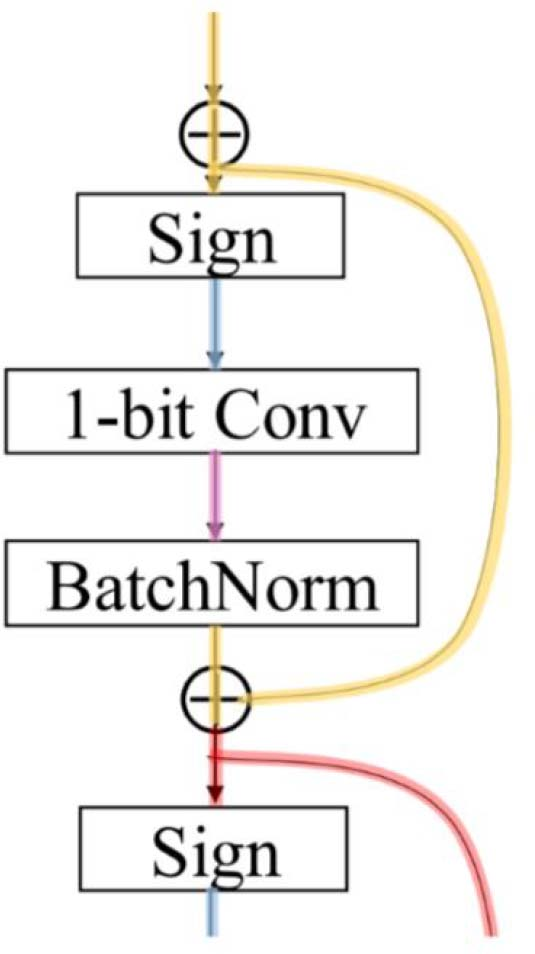
\includegraphics[width=0.25\textwidth]{Figures/BiRealNet.png}
	\caption{Exemple d'une liaison résiduale d'un BiRealNet}
	\label{fig:BiRealNet}
\end{figure}

\subsection{Topologie}
BiRealNet\cite{BiRealNetPaper} est pratiquement indépendent de la topologie elle même. Mais la présence des liaisons résiduales y induit quelques contraintes.
\newline La principale contrainte que la couche résiduale et la couche actuelle doivent avoir les même dimensions.

\subsection{Block BiRealNet}
Pour bien augmenter l'apport d'informations avec BiRealNet, la connexion résiduale est faite entre deux blocs connexes et qui vérifient la contrainte sur les dimensions.
\newline De plus, le résidu doit avoir la possibilité de varier sur un ensemble réel. C'est à dire varier sur un grands ensemble de valeurs.
\newline Un exemple concis est la figure \ref{fig:BiRealNet} qui montre une connexion résiduale pour chaque bloc de:
\begin{itemize}
	\item Quantification par signe
	\item Convolution binarisée
	\item Normalisation par Lots
\end{itemize}
En effet, selon cette figure, la connexion va être faite entre le résultat du bloc actuel et le bloc précédent.
\subsection{Liaison résiduale}
\subsubsection{Notation}
Soit $\mathcal{R}(l)$ l'ensemble de couches qui ont une liaison résiduale avec la $l^\text{ème}$ couche.
\subsubsection{Contraintes sur $\mathcal{R}(l)$}
Dans BiRealNet, la seule contrainte présente est que le réseau de neurone doit rester acyclique:
\begin{equation}
	\forall l,\forall l' \in \mathcal{R}(l), \quad l' < l
\end{equation}
\subsubsection{Equation}
La liaison résiduale induit un changement de la formule de $z^{(l)}$ trouvée dans le tableau \ref{table:AcyclicNeuralNetwork} situé dans la section \ref{Theoretical:Observations}. La nouvelle expression de $z^{(l)}$ est:
\begin{equation}\label{BiRealNet:Expression}
	z^{(l)}=\boldsymbol{W}^{(l)}\tilde{\star} a^{(l-1)}+\sum_{l' \in \mathcal{R}(l)}z^{(l')}
\end{equation}

Dans cette équation, $\tilde{\star}$ signifie que l'opérateur $\star$ est quantifié avec une quantification quelconque.
Dans la plus part des cas, $\mathcal{R}(l)$ est un singleton qui contient seulement la couche du dernier bloc, ce qui est le cas par exemple pour la figure \ref{fig:BiRealNet}

\subsection{Choix de la quantification}
Dans l'équation \eqref{BiRealNet:Expression}, nous n'avons explicité aucune quantification, et c'est l'une des avantages de BiRealNet: il est orthogonal au type de binarisation\footnote{En effet, BiRealNet est un modèle basé sur l'architecture, et ces modèles sont généralement orthogonaux aux modèles basées sur la quantification, dans le sens ou en peut créer un modèle en exploitant en même temps une quantification d'un et une architecture de l'autre.}.
\newline Ainsi, l'opérateur quantifié $\tilde{\star}$ peut être basé sur BinaryNet, XnorNet, ABCNet, etc...